\documentclass{article}
\newsavebox{\oldepsilon}
\savebox{\oldepsilon}{\ensuremath{\epsilon}}
\usepackage[minionint,mathlf,textlf]{MinionPro} % To gussy up a bit
\renewcommand*{\epsilon}{\usebox{\oldepsilon}}
\usepackage[margin=1in]{geometry}
\usepackage{graphicx} % For .eps inclusion
%\usepackage{indentfirst} % Controls indentation
\usepackage[compact]{titlesec} % For regulating spacing before section titles
\usepackage{adjustbox} % For vertically-aligned side-by-side minipages
\usepackage{array, amsmath,  mhchem}
\usepackage{hyper ref}
\usepackage{courier, subcaption}
\usepackage{multirow, enumerate}

\usepackage{float}
\restylefloat{table}

\pagenumbering{gobble} 
\setlength\parindent{0 cm}
\renewcommand{\arraystretch}{1.2}
\begin{document}
\large

MCB 135 Problem Set 1 \hfill Due Wednesday, February 11, 2015 at 2:30 PM

\section*{Problem 1: Latch (20 points)}

A diagram of a ``latch" circuit built using NAND gates is shown in Figure \ref{fig:fig1}.

\begin{figure}[htp] \centering{
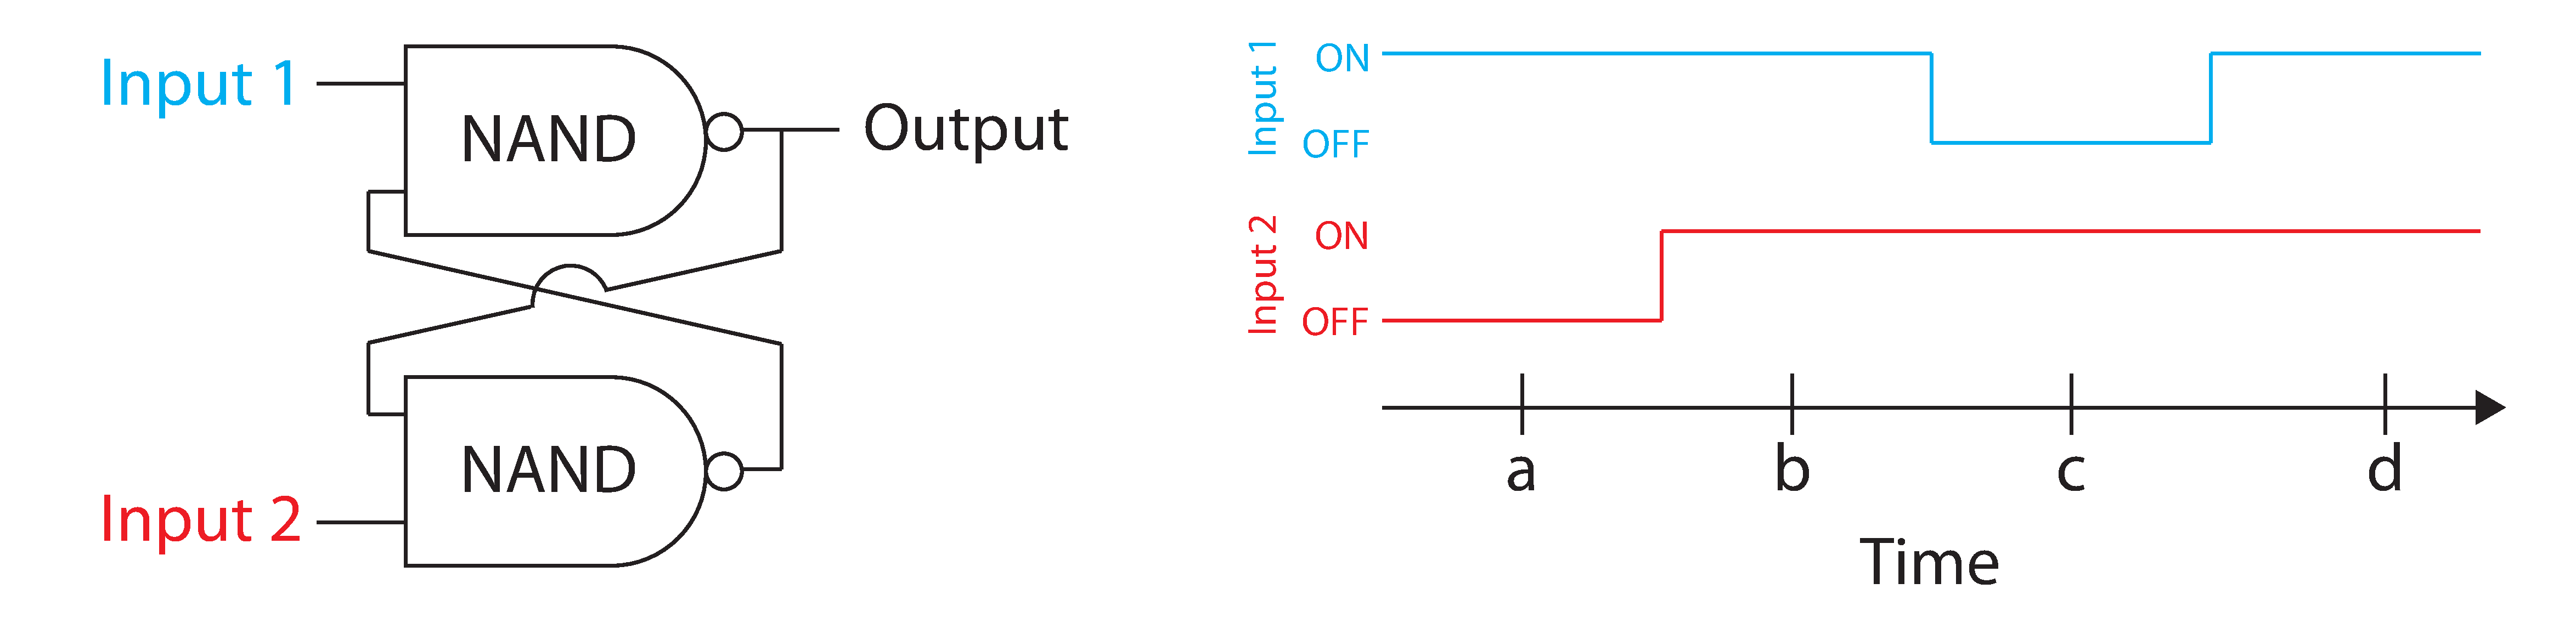
\includegraphics[width=0.8\textwidth]{latch.pdf}}
\caption{Diagram of a NAND latch circuit and timecourse of its two inputs.} \label{fig:fig1}
\end{figure}  

\begin{enumerate}[a)]
\setlength{\itemsep}{0pt}
\item For each of the four timepoints a-d indicated in Figure \ref{fig:fig1}, determine the output signal.
\item In 1-2 sentences, draw an analogy between the latch circuit and the latch of a door.
\item Suppose that a system allows an arbitrary number of NAND gates to be implemented in any configuration. Is this enough to show that the system is Turing complete? Explain.
\end{enumerate}

\section*{Problem 2: Open reaction network (Ingalls 2.4.1, 15 points)}

Suppose a reaction network is composed of the following six reactions:
\begin{eqnarray*}
\ce{ ->[k_1] \textrm{A} }\hspace{3 cm} & \ce{\textrm{A} ->[k_2] \textrm{B} + \textrm{C} }& \hspace{3 cm} \ce{ \textrm{B}  ->[k_3] }\\
\ce{ \textrm{C}  ->[k_4] 2 \textrm{D}} \hspace{3 cm} & \ce{ 2 \textrm{D}  ->[k_5] \textrm{C}} & \hspace{3 cm}  \ce{ \textrm{D}  ->[k_6]}
\end{eqnarray*}
with mass-action rate constants as indicated.

\begin{enumerate}[a)]
\setlength{\itemsep}{0pt}
\item Construct a differential equation model of the network.
\item Determine the steady-state concentrations of all species as functions of the mass-action \linebreak constants $k_i$.
\end{enumerate}

\section*{Problem 3: Moiety conservations (Ingalls 2.4.3, 15 points)}

Consider the reaction scheme in Figure \ref{fig:fig2}.

\begin{figure}[htp] \centering{
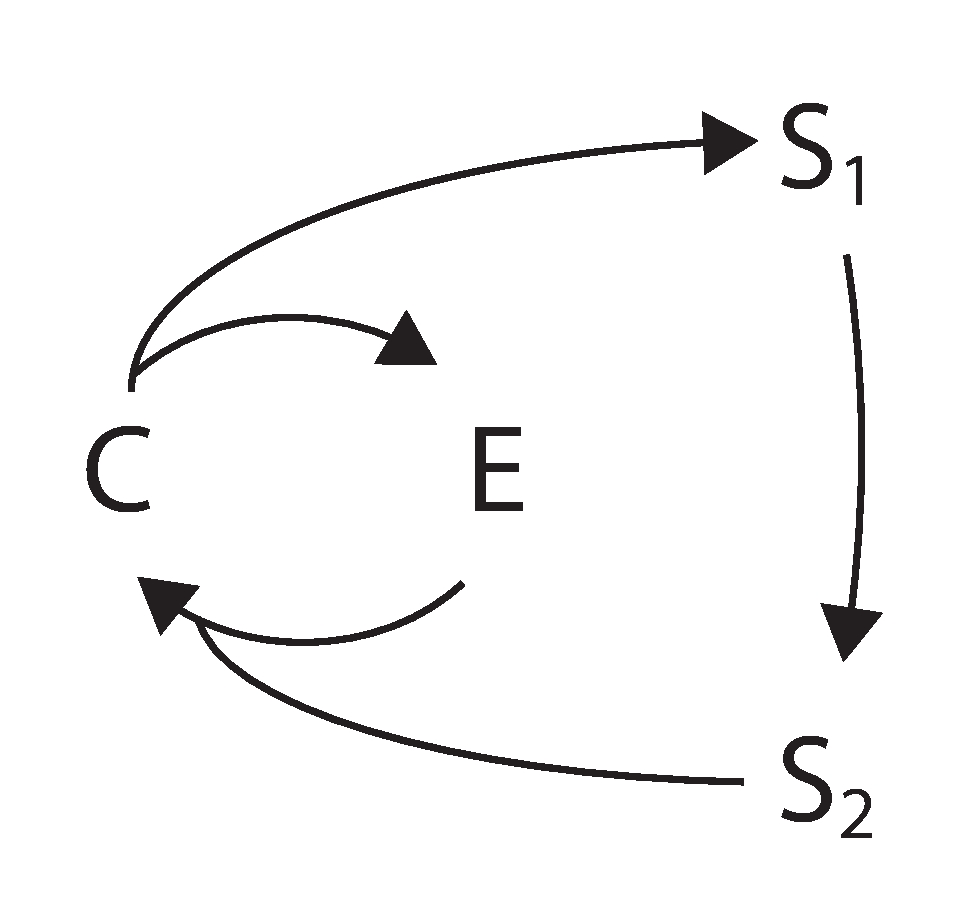
\includegraphics[width=0.2\textwidth]{moieties.pdf}}
\caption{Closed reaction network for problem 3.} \label{fig:fig2}
\end{figure}  

\begin{enumerate}[a)]
\setlength{\itemsep}{0pt}
\item Identify two moiety conservations in the network.
\item Consider an experiment in which the initial concentrations are (in mM) $s_1(0) = 3.5$, $s_2(0) = 1$,  $e(0) = 3$, and $c(0) = 0$. Suppose that the steady-state concentrations of $S_1$ and $S_2$ are $s_1^{\textrm{ss}} = 2$ mM and $s_2^{\textrm{ss}} = 1.5$ mM. Determine the steady-state concentrations of $E$ and $C$. (Note: there is no need to consider the reaction rates or network dynamics. The conclusion follows directly from the moiety conservations.)
\end{enumerate}

\section*{Problem 4: Rapid Equilibrium Approximation (Ingalls 2.4.8, 25 points)}

Consider the closed system
\begin{eqnarray*}
& \ce{\textrm{A} <=>[k_1][k_{-1}]  \textrm{B}  <=>[k_2][k_{-2}] \textrm{C}} &
\end{eqnarray*}
with mass-action rate constants as shown. Suppose the rate constants are (in min$^{-1}$) $k_1 = 0.05$, $k_2 = 0.7$, $k_{-1} = 0.005$, and $k_{-2} = 0.4$.

\begin{enumerate}[a)]
\setlength{\itemsep}{0pt}
\item Construct a differential equation model of the system. Simulate your model with initial conditions (in mM) of $A(0)=1.5$, $B(0) = 3$, and $C(0)=2$. Plot the transient and steady-state behavior of the system. You may need to make two plots to capture all of the dynamics (i.e. two different window sizes).
\item It should be clear from your simulation in part a that the system dynamics occur on two different timescales. This is also apparent in the widely separated rate constants. Use a rapid equilibrium assumption to reduce your description of the system to two differentiated equations (describing one of the original species and one combined species pool) and two algebraic equations (describing the contents of the combined pool).
\item Run a simulation of your reduced model in part b to compare with the simulation in part a. Verify that the simulation of the reduced system is in good agreement with the original, except for a short initial transient. (Note that you will have to select initial conditions for the reduced system so that the initial total concentration is in agreement with part a, and the rapid equilibrium condition is satisfied at time $t=0$.)
\end{enumerate}

\section*{Problem 5: Quasi-Steady-State Approximation (Ingalls 2.4.9, 25 points)}
Consider the reaction network
\begin{eqnarray*}
&\ce{->[k_0]  \textrm{A} ->[k_2] } \hspace{2 cm} \ce{\textrm{A} <=>[k_1][k_{-1}] \textrm{B} }&
\end{eqnarray*}
Suppose the mass-action rate constants are (in min$^{-1}$) $k_0 = 1$, $k_1 = 11$, $k_{-1} = 8$, and $k_2 = 0.2$.

\begin{enumerate}[a)]
\setlength{\itemsep}{0pt}
\item Construct a differential equation model of the system. Simulate your model with initial conditions $A(0) = 6$ mM, $B(0) = 0$ mM. Plot the transient and steady-state behavior of the system. You may need to make two plots to capture all of the dynamics (i.e., two different window sizes).
\item It should be clear from your simulation in part a that the system dynamics occur on two different timescales. This is also apparent in the widely separated rate constants. Use a quasi-steady-state assumption to reduce your description of the system by replacing a differential equation with an algebraic equation.
\item Run a simulation of your reduced model in part b to compare with the simulation in part a. Verify that the simulation of the reduced system is a good approximation of the original at steady-state, but not over the initial transient. (Note that you will have to select initial conditions for the reduced system so that the total concentration is in agreement  with part a and the quasi-steady-state condition is satisfied at time $t=0$, as in problem 4.
\end{enumerate}
\end{document}